% This article has been prepared for publication in Energy Economics in RStudio with knitr.
% According to http://www.elsevier.com/author-schemas/the-elsarticle-latex-document-class, we should be using the
% elsarticle.cls file.
% According to http://cdn.elsevier.com/assets/pdf_file/0006/109392/journal_refstyles.pdf, we should be using
% elsarticle-template-2-harv.tex as the template for the text.
% Furthermore, we should be using model2-names.bst for the bibliographic references.
% The approach here is to load the frontmatter and backmatter from elsarticle-template-2-harv.tex
% both ahead of and behind the text for our paper.
% -- Matthew Kuperus Heun, 2013-01-18

%% This is file `elsarticle-template-2-harv.tex',
%%
%% Copyright 2009 Elsevier Ltd
%%
%% This file is part of the 'Elsarticle Bundle'.
%% ---------------------------------------------
%%
%% It may be distributed under the conditions of the LaTeX Project Public
%% License, either version 1.2 of this license or (at your option) any
%% later version.  The latest version of this license is in
%%    http://www.latex-project.org/lppl.txt
%% and version 1.2 or later is part of all distributions of LaTeX
%% version 1999/12/01 or later.
%%
%% The list of all files belonging to the 'Elsarticle Bundle' is
%% given in the file `manifest.txt'.
%%
%% Template article for Elsevier's document class `elsarticle'
%% with harvard style bibliographic references
%%
%% $Id: elsarticle-template-2-harv.tex 155 2009-10-08 05:35:05Z rishi $
%% $URL: http://lenova.river-valley.com/svn/elsbst/trunk/elsarticle-template-2-harv.tex $
%%
\documentclass[preprint,authoryear,12pt]{elsarticle}\usepackage{graphicx, color}
%% maxwidth is the original width if it is less than linewidth
%% otherwise use linewidth (to make sure the graphics do not exceed the margin)
\makeatletter
\def\maxwidth{ %
  \ifdim\Gin@nat@width>\linewidth
    \linewidth
  \else
    \Gin@nat@width
  \fi
}
\makeatother

\IfFileExists{upquote.sty}{\usepackage{upquote}}{}
\definecolor{fgcolor}{rgb}{0.2, 0.2, 0.2}
\newcommand{\hlnumber}[1]{\textcolor[rgb]{0,0,0}{#1}}%
\newcommand{\hlfunctioncall}[1]{\textcolor[rgb]{0.501960784313725,0,0.329411764705882}{\textbf{#1}}}%
\newcommand{\hlstring}[1]{\textcolor[rgb]{0.6,0.6,1}{#1}}%
\newcommand{\hlkeyword}[1]{\textcolor[rgb]{0,0,0}{\textbf{#1}}}%
\newcommand{\hlargument}[1]{\textcolor[rgb]{0.690196078431373,0.250980392156863,0.0196078431372549}{#1}}%
\newcommand{\hlcomment}[1]{\textcolor[rgb]{0.180392156862745,0.6,0.341176470588235}{#1}}%
\newcommand{\hlroxygencomment}[1]{\textcolor[rgb]{0.43921568627451,0.47843137254902,0.701960784313725}{#1}}%
\newcommand{\hlformalargs}[1]{\textcolor[rgb]{0.690196078431373,0.250980392156863,0.0196078431372549}{#1}}%
\newcommand{\hleqformalargs}[1]{\textcolor[rgb]{0.690196078431373,0.250980392156863,0.0196078431372549}{#1}}%
\newcommand{\hlassignement}[1]{\textcolor[rgb]{0,0,0}{\textbf{#1}}}%
\newcommand{\hlpackage}[1]{\textcolor[rgb]{0.588235294117647,0.709803921568627,0.145098039215686}{#1}}%
\newcommand{\hlslot}[1]{\textit{#1}}%
\newcommand{\hlsymbol}[1]{\textcolor[rgb]{0,0,0}{#1}}%
\newcommand{\hlprompt}[1]{\textcolor[rgb]{0.2,0.2,0.2}{#1}}%

\usepackage{framed}
\makeatletter
\newenvironment{kframe}{%
 \def\at@end@of@kframe{}%
 \ifinner\ifhmode%
  \def\at@end@of@kframe{\end{minipage}}%
  \begin{minipage}{\columnwidth}%
 \fi\fi%
 \def\FrameCommand##1{\hskip\@totalleftmargin \hskip-\fboxsep
 \colorbox{shadecolor}{##1}\hskip-\fboxsep
     % There is no \\@totalrightmargin, so:
     \hskip-\linewidth \hskip-\@totalleftmargin \hskip\columnwidth}%
 \MakeFramed {\advance\hsize-\width
   \@totalleftmargin\z@ \linewidth\hsize
   \@setminipage}}%
 {\par\unskip\endMakeFramed%
 \at@end@of@kframe}
\makeatother

\definecolor{shadecolor}{rgb}{.97, .97, .97}
\definecolor{messagecolor}{rgb}{0, 0, 0}
\definecolor{warningcolor}{rgb}{1, 0, 1}
\definecolor{errorcolor}{rgb}{1, 0, 0}
\newenvironment{knitrout}{}{} % an empty environment to be redefined in TeX

\usepackage{alltt}

%% Use the option review to obtain double line spacing
%% \documentclass[authoryear,preprint,review,12pt]{elsarticle}

%% Use the options 1p,twocolumn; 3p; 3p,twocolumn; 5p; or 5p,twocolumn
%% for a journal layout:
%% \documentclass[final,authoryear,1p,times]{elsarticle}
%% \documentclass[final,authoryear,1p,times,twocolumn]{elsarticle}
%% \documentclass[final,authoryear,3p,times]{elsarticle}
%% \documentclass[final,authoryear,3p,times,twocolumn]{elsarticle}
%% \documentclass[final,authoryear,5p,times]{elsarticle}
%% \documentclass[final,authoryear,5p,times,twocolumn]{elsarticle}

%% if you use PostScript figures in your article
%% use the graphics package for simple commands
%% \usepackage{graphics}
%% or use the graphicx package for more complicated commands
%% \usepackage{graphicx}
%% or use the epsfig package if you prefer to use the old commands
%% \usepackage{epsfig}

%% The amssymb package provides various useful mathematical symbols
\usepackage{amssymb}
%% The amsthm package provides extended theorem environments
%% \usepackage{amsthm}

%% The lineno packages adds line numbers. Start line numbering with
%% \begin{linenumbers}, end it with \end{linenumbers}. Or switch it on
%% for the whole article with \linenumbers after \end{frontmatter}.
%% \usepackage{lineno}

%% natbib.sty is loaded by default. However, natbib options can be
%% provided with \biboptions{...} command. Following options are
%% valid:

%%   round  -  round parentheses are used (default)
%%   square -  square brackets are used   [option]
%%   curly  -  curly braces are used      {option}
%%   angle  -  angle brackets are used    <option>
%%   semicolon  -  multiple citations separated by semi-colon (default)
%%   colon  - same as semicolon, an earlier confusion
%%   comma  -  separated by comma
%%   authoryear - selects author-year citations (default)
%%   numbers-  selects numerical citations
%%   super  -  numerical citations as superscripts
%%   sort   -  sorts multiple citations according to order in ref. list
%%   sort&compress   -  like sort, but also compresses numerical citations
%%   compress - compresses without sorting
%%   longnamesfirst  -  makes first citation full author list
%%
%% \biboptions{longnamesfirst,comma}

% \biboptions{}

\journal{Energy Economics}

\begin{document}

\begin{frontmatter}

%% Title, authors and addresses

%% use the tnoteref command within \title for footnotes;
%% use the tnotetext command for the associated footnote;
%% use the fnref command within \author or \address for footnotes;
%% use the fntext command for the associated footnote;
%% use the corref command within \author for corresponding author footnotes;
%% use the cortext command for the associated footnote;
%% use the ead command for the email address,
%% and the form \ead[url] for the home page:
%%
%% \title{Title\tnoteref{label1}}
%% \tnotetext[label1]{}
%% \author{Name\corref{cor1}\fnref{label2}}
%% \ead{email address}
%% \ead[url]{home page}
%% \fntext[label2]{}
%% \cortext[cor1]{}
%% \address{Address\fnref{label3}}
%% \fntext[label3]{}

\title{Empirical Analysis of the Role of Energy in Economic Growth}

%% use optional labels to link authors explicitly to addresses:
%% \author[label1,label2]{<author name>}
%% \address[label1]{<address>}
%% \address[label2]{<address>}

\author[Calvin]{Caleb Reese}
\author[Calvin]{Lucas Timmer}
\author[Calvin]{Matthew Kuperus Heun \corref{cor1}}
\ead{mkh2@calvin.edu, tel: +1 (616) 526-6663, fax: +1 (616) 526-6501}

\cortext[cor1]{Corresponding author}
\address[Calvin]{Engineering Department, Calvin College, Grand Rapids, MI 49546, USA}

\begin{abstract}
%% Text of abstract
*********** Add abstract ***********
\end{abstract}

\begin{keyword}
%% keywords here, in the form: keyword \sep keyword
economic growth \sep energy \sep cobb-douglas \sep CES \sep LINEX
%% MSC codes here, in the form: \MSC code \sep code
%% or \MSC[2008] code \sep code (2000 is the default)
\end{keyword}

\end{frontmatter}

% \linenumbers
%% main text





\begin{knitrout}
\definecolor{shadecolor}{rgb}{0.969, 0.969, 0.969}\color{fgcolor}\begin{kframe}
\begin{alltt}
fileName <- \hlstring{"data/USData.txt"}

\hlcomment{# Read the data file as a table with a header.  }
\hlcomment{## dataTable is a poor name.  Name it after contents, unless this is the }
\hlcomment{## start of a script where this will be provided at the command line.}
dataTable <- \hlfunctioncall{read.table}(fileName, header = TRUE)

\hlcomment{# Identifies the header names associated with dataTable}
\hlfunctioncall{names}(dataTable)
\end{alltt}
\begin{verbatim}
 [1] "Year"                                     
 [2] "GDP.Millionsofreal2005USdollars."         
 [3] "Labour.Millionsofhoursworked."            
 [4] "CapitalStock.Millionsofreal2005USdollars."
 [5] "Thermalenergy.TJ."                        
 [6] "Exergy.TJ."                               
 [7] "UsefulWork.TJ."                           
 [8] "iYear"                                    
 [9] "iGDP"                                     
[10] "iLabor"                                   
[11] "iCapStk"                                  
[12] "iQ"                                       
[13] "iX"                                       
[14] "iU"                                       
\end{verbatim}
\end{kframe}
\end{knitrout}


\section{Cobb-Douglas Without Energy}

\begin{knitrout}
\definecolor{shadecolor}{rgb}{0.969, 0.969, 0.969}\color{fgcolor}\begin{kframe}
\begin{alltt}
\hlcomment{# Establish guess values for alpha and lambda.}
lambdaGuess <- 0.0 \hlcomment{# guessing lambda = 0 means there is no technological progress.}
alphaGuess <- 0.3 \hlcomment{# a typical value for alpha, the coefficient on capital stock}

\hlcomment{# Runs a non-linear least squares fit to the data. We've replaced beta with 1-alpha for simplicity.}
modelCD <- \hlfunctioncall{nls}(iGDP ~ \hlfunctioncall{exp}(lambda*iYear) * iCapStk^alpha * iLabor^(1 - alpha), 
               start=(\hlfunctioncall{list}(lambda=lambdaGuess,alpha=alphaGuess)),
               data=dataTable)

\hlcomment{# Checks validity of the model. AIC stands for Akaike's Information Criterion.}
aicCD  <- \hlfunctioncall{AIC}(modelCD, k=2); aicCD
\end{alltt}
\begin{verbatim}
[1] -163
\end{verbatim}
\begin{alltt}

summaryCD <- \hlfunctioncall{summary}(modelCD) \hlcomment{# Gives the nls summary table.}
\hlfunctioncall{print}(summaryCD)
\end{alltt}
\begin{verbatim}

Formula: iGDP ~ exp(lambda * iYear) * iCapStk^alpha * iLabor^(1 - alpha)

Parameters:
       Estimate Std. Error t value Pr(>|t|)
lambda 0.010256   0.000682   15.03  1.7e-15
alpha  0.270030   0.028311    9.54  1.4e-10

Residual standard error: 0.0178 on 30 degrees of freedom

Number of iterations to convergence: 4 
Achieved convergence tolerance: 3.81e-07 
\end{verbatim}
\begin{alltt}
ciCD <- \hlfunctioncall{confint}(modelCD, level = 0.95); ciCD \hlcomment{# Displays confidence intervals for the CD model.}
\end{alltt}


{\ttfamily\noindent\itshape\color{messagecolor}{Waiting for profiling to be done...}}\begin{verbatim}
           2.5%   97.5%
lambda 0.008862 0.01164
alpha  0.212405 0.32785
\end{verbatim}
\begin{alltt}

\hlcomment{# Calculate beta and its confidence interval and report it.}
alpha <- \hlfunctioncall{as.numeric}(\hlfunctioncall{coef}(modelCD)[\hlstring{"alpha"}])
beta <- 1.0 - alpha
beta.est <- \hlfunctioncall{deltaMethod}(modelCD, \hlstring{"1 - alpha"}); beta.est # Estimates beta and its standard \hlfunctioncall{error} (SE).
\end{alltt}
\begin{verbatim}
          Estimate      SE
1 - alpha     0.73 0.02831
\end{verbatim}
\begin{alltt}
\hlcomment{# Now calculate a confidence interval on beta}
dofCD <- summaryCD$df[2]; dofCD \hlcomment{# Gives the degrees of freedom for the model.}
\end{alltt}
\begin{verbatim}
[1] 30
\end{verbatim}
\begin{alltt}
tvalCD <- \hlfunctioncall{qt}(0.975, df = dofCD); tvalCD
\end{alltt}
\begin{verbatim}
[1] 2.042
\end{verbatim}
\begin{alltt}
betaCICD <- \hlfunctioncall{with}(beta.est, Estimate + \hlfunctioncall{c}(-1.0, 1.0) * tvalCD * SE); betaCICD \hlcomment{# Gives the confidence interval on beta.}
\end{alltt}
\begin{verbatim}
[1] 0.6722 0.7878
\end{verbatim}
\begin{alltt}

\hlfunctioncall{coef}(modelCD)
\end{alltt}
\begin{verbatim}
 lambda   alpha 
0.01026 0.27003 
\end{verbatim}
\begin{alltt}

\hlcomment{# Combine all estimates and their confidence intervals into data frames with intelligent row names}
estCD <- \hlfunctioncall{data.frame}(lambda = \hlfunctioncall{coef}(modelCD)[\hlstring{"lambda"}], alpha = \hlfunctioncall{coef}(modelCD)[\hlstring{"alpha"}], beta = beta, gamma = 0)
\hlfunctioncall{row.names}(estCD) <- \hlstring{"Cobb-Douglas"}
\hlcomment{#row.names(estCD) <- "Cobb-Douglas: $y = e^\{\textbackslash{}\textbackslash{}lambda t\}k^\{\textbackslash{}\textbackslash{}alpha\}l^\{\textbackslash{}\textbackslash{}beta\}$"}
\hlcomment{# The [1] subscripts pick off the lower confidence interval}
lowerCD <- \hlfunctioncall{data.frame}(lambda = ciCD[\hlstring{"lambda"},\hlstring{"2.5%"}], alpha = ciCD[\hlstring{"alpha"}, \hlstring{"2.5%"}], beta = betaCICD[1], gamma = NA) 
\hlfunctioncall{row.names}(lowerCD) <- \hlstring{"- 95% CI"}
\hlcomment{# The [2] subscripts pick off the lower confidence interval}
upperCD <- \hlfunctioncall{data.frame}(lambda = ciCD[\hlstring{"lambda"},\hlstring{"97.5%"}], alpha = ciCD[\hlstring{"alpha"}, \hlstring{"97.5%"}], beta = betaCICD[2], gamma = NA)
\hlfunctioncall{row.names}(upperCD) <- \hlstring{"+ 95% CI"}

\hlcomment{# Now create the data for a table.}
dataCD <- \hlfunctioncall{rbind}(lowerCD, estCD, upperCD); dataCD
\end{alltt}
\begin{verbatim}
               lambda  alpha   beta gamma
- 95% CI     0.008862 0.2124 0.6722    NA
Cobb-Douglas 0.010256 0.2700 0.7300     0
+ 95% CI     0.011645 0.3279 0.7878    NA
\end{verbatim}
\begin{alltt}
\hlfunctioncall{colnames}(dataCD) <- \hlfunctioncall{c}(\hlstring{"$\textbackslash{}\textbackslash{}lambda$"}, \hlstring{"$\textbackslash{}\textbackslash{}alpha$"}, \hlstring{"$\textbackslash{}\textbackslash{}beta$"}, \hlstring{"$\textbackslash{}\textbackslash{}gamma$"})
tableCD <- \hlfunctioncall{xtable}(dataCD, caption=\hlstring{"U.S. Cobb-Douglas, 1980-2011"}, digit = \hlfunctioncall{c}(4, 4, 2, 2, 1))
\end{alltt}
\end{kframe}
\end{knitrout}


\begin{kframe}
\begin{alltt}
\hlfunctioncall{print}(tableCD, caption.placement=\hlstring{"top"})
\end{alltt}
\end{kframe}% latex table generated in R 2.15.2 by xtable 1.7-0 package
% Fri Jan 18 22:11:08 2013
\begin{table}[ht]
\begin{center}
\caption{U.S. Cobb-Douglas, 1980-2011}
\begin{tabular}{rrrrr}
  \hline
 & \$$\backslash$lambda\$ & \$$\backslash$alpha\$ & \$$\backslash$beta\$ & \$$\backslash$gamma\$ \\ 
  \hline
- 95\% CI & 0.0089 & 0.21 & 0.67 &  \\ 
  Cobb-Douglas & 0.0103 & 0.27 & 0.73 & 0.0 \\ 
  + 95\% CI & 0.0116 & 0.33 & 0.79 &  \\ 
   \hline
\end{tabular}
\end{center}
\end{table}
\begin{kframe}\begin{alltt}
\hlcomment{# According to http://cran.r-project.org/web/packages/xtable/vignettes/xtableGallery.pdf, Section 3.1, I should }
\hlcomment{# be able to use the "sanitize.text.function" parameter to allow markup in column headers. But this next}
\hlcomment{# line is not working at the present time. --MKH, 18 Jan 2012.}
\hlcomment{# print(tableCD, caption.placement="top", sanitize.text.function = function(x)\{x\})}
\end{alltt}
\end{kframe}


\section{Cobb-Douglas With Energy}

\begin{knitrout}
\definecolor{shadecolor}{rgb}{0.969, 0.969, 0.969}\color{fgcolor}\begin{kframe}
\begin{alltt}
\hlcomment{###############################}
\hlcomment{# This function fits the Cobb Douglas production function including energy to historical data}
\hlcomment{# The functional form is}
\hlcomment{#}
\hlcomment{# iGDP = exp(lambda * itime) * iCapStk^alpha * iLabor^beta * iEnergy^gamma}
\hlcomment{# }
\hlcomment{# iYear: time indexed to 0.0 at the first year [years since beginning of data set]}
\hlcomment{# iGDP = time series GDP data indexed to 1.0 at the first year [-]}
\hlcomment{# iCapStk = time series capital stock data indexed to 1.0 at the first year [-]}
\hlcomment{# iLabor = time series labor data indexed to 1.0 at the first year [-]}
\hlcomment{# iEnergy = time series energy data indexed to 1.0 at the first year [-]. }
\hlcomment{#      This may be any of heat (iQ), exergy (iX), or useful work (iU).}
\hlcomment{# }
\hlcomment{# returns a data object containing three rows and 5 columns.}
\hlcomment{#   col 1: lambda}
\hlcomment{#   col 2: alpha}
\hlcomment{#   col 3: beta}
\hlcomment{#   col 4: gamma}
\hlcomment{#   row 1: -95% CI for each parameter}
\hlcomment{#   row 2: estimate for each parameter}
\hlcomment{#   row 3: +95% CI for each parameter}
\hlcomment{#}
\hlcomment{# dataTable is the table to be used for this curve fit}
\hlcomment{# iEnergy is the name of the column to be used for energy.}
\hlcomment{#   This may be any of heat (iQ), exergy (iX), or useful work (iU).}
\hlcomment{##}
cobbDouglasEnergy <- \hlfunctioncall{function}(dataTable, iEnergy)\{
\hlcomment{  # Reparameterize to ensure that we meet the constraints:}
\hlcomment{  # * alpha + beta + gamma = 1.0.}
\hlcomment{  # * alpha, beta, and gamma are all between 0.0 and 1.0.}
\hlcomment{  # To do this, we reparameterize as}
\hlcomment{  # * 0 < a < 1}
\hlcomment{  # * 0 < b < 1}
\hlcomment{  # * alpha = min(a, b)}
\hlcomment{  # * beta = b - a}
\hlcomment{  # * gamma = 1 - max(a, b)}
  energyName = \hlfunctioncall{names}(iEnergy) \hlcomment{#grabs the name of the energy column}
  lambdaGuess <- 0.0 \hlcomment{# guessing lambda = 0 means there is no technological progress.}
  alphaGuess <- 0.3 \hlcomment{# a typical value for alpha}
  betaGuess <- 0.7 \hlcomment{# a typical value for beta}
  modelCDe <- \hlfunctioncall{nls}(iGDP ~ \hlfunctioncall{exp}(lambda*iYear) * 
                    iCapStk^\hlfunctioncall{min}(a,b) * iLabor^\hlfunctioncall{abs}(b-a) * 
                    iEnergy^(1.0 - \hlfunctioncall{max}(a,b)), 
                  algorithm = \hlstring{"port"},
                  start = \hlfunctioncall{list}(lambda=lambdaGuess, a=alphaGuess, b=alphaGuess+betaGuess),
                  lower = \hlfunctioncall{list}(lambda=-Inf, a=0, b=0),
                  upper = \hlfunctioncall{list}(lambda=Inf, a=1, b=1),
                  data = dataTable)
  aicCDe <- \hlfunctioncall{AIC}(modelCDe, k=2) \hlcomment{# Checks validity of the model. AIC stands for Akaike's Information Criterion}
  \hlfunctioncall{print}(aicCDe)
  
  summaryCDe <- \hlfunctioncall{summary}(modelCDe) \hlcomment{# Gives the nls summary table}
  \hlfunctioncall{print}(summaryCDe)
  
\hlcomment{  # Provides confidence intervals on lambda, a, and b. But, we need CIs on alpha and beta.}
  ciCDe <- \hlfunctioncall{confint}(modelCDe, level = 0.95)
  \hlfunctioncall{print}(ciCDe)
  
  a <- \hlfunctioncall{as.numeric}(\hlfunctioncall{coef}(modelCDe)[\hlstring{"a"}])
  b <- \hlfunctioncall{as.numeric}(\hlfunctioncall{coef}(modelCDe)[\hlstring{"b"}])
  lambda <- \hlfunctioncall{as.numeric}(\hlfunctioncall{coef}(modelCDe)[\hlstring{"lambda"}])
  alpha <- a
  beta <- b - a
  gamma <- 1.0 - alpha - beta
  
\hlcomment{  # Report results with SE}
  beta.est <- \hlfunctioncall{deltaMethod}(modelCDe, \hlstring{"b-a"}) # Reports results for beta, because beta = b - a.
  gamma.est <- \hlfunctioncall{deltaMethod}(modelCDe, \hlstring{"1-b"}) # Reports results for gamma, because gamma = 1 - b.
  
\hlcomment{  # Now calculate confidence intervals.}
  dofCDe <- summaryCDe$df[2] \hlcomment{# Gives the degrees of freedom for the model.}
  \hlfunctioncall{print}(dofCDe)
  tvalCDe <- \hlfunctioncall{qt}(0.975, df = dofCDe)
  \hlfunctioncall{print}(tvalCDe)
  betaCICDe <- \hlfunctioncall{with}(beta.est, Estimate + \hlfunctioncall{c}(-1.0, 1.0) * tvalCDe * SE) \hlcomment{# Gives the confidence interval on beta.}
  \hlfunctioncall{print}(betaCICDe)
  gammaCICDe <- \hlfunctioncall{with}(gamma.est, Estimate + \hlfunctioncall{c}(-1.0, 1.0) * tvalCDe * SE) \hlcomment{# Gives the confidence interval on alpha.}
  \hlfunctioncall{print}(gammaCICDe)
  
\hlcomment{  # Combine all estimates and their confidence intervals into data frames with intelligent row names}
  estCDe <- \hlfunctioncall{data.frame}(lambda = lambda, alpha = alpha, beta = beta, gamma = gamma)
  \hlfunctioncall{print}(estCDe);
\hlcomment{  #row.names(estCDe) <- "Cobb-Douglas with e: $y = e^\{\textbackslash{}\textbackslash{}lambda t\}k^\{\textbackslash{}\textbackslash{}alpha\}l^\{\textbackslash{}\textbackslash{}beta\}e^\{\textbackslash{}\textbackslash{}gamma\}$"}
  \hlfunctioncall{row.names}(estCDe) <- \hlfunctioncall{paste}(\hlstring{"Cobb-Douglas with "}, energyName, sep=\hlstring{""})
\hlcomment{  # The [1] subscripts pick off the lower confidence interval}
  lowerCDe <- \hlfunctioncall{data.frame}(lambda = ciCDe[\hlstring{"lambda"},\hlstring{"2.5%"}], alpha = ciCDe[\hlstring{"a"}, \hlstring{"2.5%"}], beta = betaCICDe[1], gamma = gammaCICDe[1])
  \hlfunctioncall{row.names}(lowerCDe) <- \hlstring{"- 95% CI"}
\hlcomment{  # The [2] subscripts pick off the lower confidence interval}
  upperCDe <- \hlfunctioncall{data.frame}(lambda = ciCDe[\hlstring{"lambda"},\hlstring{"97.5%"}], alpha = ciCDe[\hlstring{"a"}, \hlstring{"97.5%"}], beta = betaCICDe[2], gamma = gammaCICDe[2])
  \hlfunctioncall{row.names}(upperCDe) <- \hlstring{"+ 95% CI"}
  
\hlcomment{  # Now create the data for a table.}
  dataCDe <- \hlfunctioncall{rbind}(lowerCDe, estCDe, upperCDe)
  \hlfunctioncall{print}(dataCDe)
  
  \hlfunctioncall{return}(dataCDe)
\}
\end{alltt}
\end{kframe}
\end{knitrout}


\subsection{Cobb-Douglas with Q}

\begin{knitrout}
\definecolor{shadecolor}{rgb}{0.969, 0.969, 0.969}\color{fgcolor}\begin{kframe}
\begin{alltt}
dataCDe <- \hlfunctioncall{cobbDouglasEnergy}(dataTable, dataTable[\hlstring{"iQ"}])
\end{alltt}
\begin{verbatim}
[1] -161.1

Formula: iGDP ~ exp(lambda * iYear) * iCapStk^min(a, b) * iLabor^abs(b - 
    a) * iEnergy^(1 - max(a, b))

Parameters:
       Estimate Std. Error t value Pr(>|t|)
lambda  0.01049    0.00108    9.67  1.4e-10
a       0.26322    0.03795    6.94  1.3e-07
b       0.97890    0.07647   12.80  1.9e-13

Residual standard error: 0.0181 on 29 degrees of freedom

Algorithm "port", convergence message: relative convergence (4) 
\end{verbatim}


{\ttfamily\noindent\itshape\color{messagecolor}{Waiting for profiling to be done...}}\begin{verbatim}
          2.5%  97.5%
lambda 0.00885 0.0127
a      0.18580 0.3283
b      0.82175     NA
[1] 29
[1] 2.045
[1] 0.5947 0.8367
[1] -0.1353  0.1775
   lambda  alpha   beta  gamma
1 0.01049 0.2632 0.7157 0.0211
                      lambda  alpha   beta   gamma
- 95% CI             0.00885 0.1858 0.5947 -0.1353
Cobb-Douglas with iQ 0.01049 0.2632 0.7157  0.0211
+ 95% CI             0.01270 0.3283 0.8367  0.1775
\end{verbatim}
\begin{alltt}
tableCDe <- \hlfunctioncall{xtable}(dataCDe, caption=\hlstring{"U.S. 1980-2011."}, digit = \hlfunctioncall{c}(4, 4, 2, 2, 3))
\hlcomment{#estCDe <- dataCDe[2]}
\hlcomment{#dataAll <- rbind(estCD, estCDe); dataAll}
\hlcomment{#tableAll <- xtable(dataAll, caption="U.S. 1980-2011, All Models.", digit = c(4, 4, 2, 2, 3))}
\end{alltt}
\end{kframe}
\end{knitrout}


\begin{kframe}
\begin{alltt}

\hlfunctioncall{print}(tableCDe, caption.placement=\hlstring{"top"})
\end{alltt}
\end{kframe}% latex table generated in R 2.15.2 by xtable 1.7-0 package
% Fri Jan 18 22:11:08 2013
\begin{table}[ht]
\begin{center}
\caption{U.S. 1980-2011.}
\begin{tabular}{rrrrr}
  \hline
 & lambda & alpha & beta & gamma \\ 
  \hline
- 95\% CI & 0.0089 & 0.19 & 0.59 & -0.135 \\ 
  Cobb-Douglas with iQ & 0.0105 & 0.26 & 0.72 & 0.021 \\ 
  + 95\% CI & 0.0127 & 0.33 & 0.84 & 0.177 \\ 
   \hline
\end{tabular}
\end{center}
\end{table}
\begin{kframe}\begin{alltt}
\hlcomment{# According to http://cran.r-project.org/web/packages/xtable/vignettes/xtableGallery.pdf, Section 3.1, I should }
\hlcomment{# be able to use the "sanitize.text.function" parameter to allow markup in column headers. But this next}
\hlcomment{# line is not working at the present time. --MKH, 18 Jan 2012.}
\hlcomment{# print(tableCDe, sanitize.text.function = function(x)\{x\})}

\hlcomment{#print(tableAll, caption.placement="top")}
\end{alltt}
\end{kframe}


\subsection{Cobb-Douglas With X}

\begin{knitrout}
\definecolor{shadecolor}{rgb}{0.969, 0.969, 0.969}\color{fgcolor}\begin{kframe}
\begin{alltt}
dataCDx <- \hlfunctioncall{cobbDouglasEnergy}(dataTable, dataTable[\hlstring{"iX"}])
\end{alltt}
\begin{verbatim}
[1] -161.4

Formula: iGDP ~ exp(lambda * iYear) * iCapStk^min(a, b) * iLabor^abs(b - 
    a) * iEnergy^(1 - max(a, b))

Parameters:
       Estimate Std. Error t value Pr(>|t|)
lambda  0.01071    0.00105   10.16  4.6e-11
a       0.25689    0.03666    7.01  1.0e-07
b       0.95700    0.07467   12.82  1.8e-13

Residual standard error: 0.018 on 29 degrees of freedom

Algorithm "port", convergence message: relative convergence (4) 
\end{verbatim}


{\ttfamily\noindent\itshape\color{messagecolor}{Waiting for profiling to be done...}}\begin{verbatim}
           2.5%   97.5%
lambda 0.008902 0.01287
a      0.182137 0.32622
b      0.803506      NA
[1] 29
[1] 2.045
[1] 0.5791 0.8211
[1] -0.1097  0.1957
   lambda  alpha   beta gamma
1 0.01071 0.2569 0.7001 0.043
                       lambda  alpha   beta   gamma
- 95% CI             0.008902 0.1821 0.5791 -0.1097
Cobb-Douglas with iX 0.010714 0.2569 0.7001  0.0430
+ 95% CI             0.012867 0.3262 0.8211  0.1957
\end{verbatim}
\begin{alltt}
tableCDx <- \hlfunctioncall{xtable}(dataCDx, caption=\hlstring{"U.S. 1980-2011."}, digit = \hlfunctioncall{c}(4, 4, 2, 2, 3))
\end{alltt}
\end{kframe}
\end{knitrout}


\begin{kframe}
\begin{alltt}
\hlfunctioncall{print}(tableCDx, caption.placement=\hlstring{"top"})
\end{alltt}
\end{kframe}% latex table generated in R 2.15.2 by xtable 1.7-0 package
% Fri Jan 18 22:11:09 2013
\begin{table}[ht]
\begin{center}
\caption{U.S. 1980-2011.}
\begin{tabular}{rrrrr}
  \hline
 & lambda & alpha & beta & gamma \\ 
  \hline
- 95\% CI & 0.0089 & 0.18 & 0.58 & -0.110 \\ 
  Cobb-Douglas with iX & 0.0107 & 0.26 & 0.70 & 0.043 \\ 
  + 95\% CI & 0.0129 & 0.33 & 0.82 & 0.196 \\ 
   \hline
\end{tabular}
\end{center}
\end{table}



\subsection{Cobb-Douglas With U}

\begin{knitrout}
\definecolor{shadecolor}{rgb}{0.969, 0.969, 0.969}\color{fgcolor}\begin{kframe}
\begin{alltt}
dataCDu <- \hlfunctioncall{cobbDouglasEnergy}(dataTable, dataTable[\hlstring{"iU"}])
\end{alltt}


{\ttfamily\noindent\bfseries\color{errorcolor}{Error: Missing value or an infinity produced when evaluating the model}}\begin{alltt}
tableCDu <- \hlfunctioncall{xtable}(dataCDu, caption=\hlstring{"U.S. 1980-2011."}, digit = \hlfunctioncall{c}(4, 4, 2, 2, 3))
\end{alltt}


{\ttfamily\noindent\bfseries\color{errorcolor}{Error: object 'dataCDu' not found}}\end{kframe}
\end{knitrout}


\begin{kframe}
\begin{alltt}
\hlfunctioncall{print}(tableCDu, caption.placement=\hlstring{"top"})
\end{alltt}


{\ttfamily\noindent\bfseries\color{errorcolor}{Error: error in evaluating the argument 'x' in selecting a method for function 'print': Error: object 'tableCDu' not found}}\end{kframe}





An issue arrises in this example because contraining $\alpha$ and $\beta$ is not sufficient to 
guarantee that $\gamma$ is properly constrained.

\begin{knitrout}
\definecolor{shadecolor}{rgb}{0.969, 0.969, 0.969}\color{fgcolor}\begin{kframe}
\begin{alltt}
\hlcomment{# Establish guess values for alpha, beta, and lambda.}
lambdaGuess <- 0.0 \hlcomment{# guessing lambda = 0 means there is no technological progress.}
alphaGuess <- 0.2 \hlcomment{# a typical value for alpha}
betaGuess <- 0.6 \hlcomment{# a typical value for beta}
gammaGuess <- 0.01 \hlcomment{# a nice low value}

\hlcomment{# Runs a non-linear least squares fit to the data with constraints}
modelCDU <- \hlfunctioncall{nls}(iGDP ~ \hlfunctioncall{exp}(lambda*iYear) * iCapStk^alpha * iLabor^beta * iU^(1.0 - alpha - beta), 
                algorithm=\hlstring{"port"},
                start = \hlfunctioncall{list}(lambda=lambdaGuess, alpha=alphaGuess, beta=betaGuess),
                lower = \hlfunctioncall{list}(lambda=-Inf, alpha=0, beta=0),
                upper = \hlfunctioncall{list}(lambda=Inf, alpha=1, beta=1),
                data=dataTable)

\hlcomment{# Gives the nls summary table}
\hlfunctioncall{summary}(modelCDU)
\end{alltt}
\begin{verbatim}

Formula: iGDP ~ exp(lambda * iYear) * iCapStk^alpha * iLabor^beta * iU^(1 - 
    alpha - beta)

Parameters:
       Estimate Std. Error t value Pr(>|t|)
lambda  0.00920    0.00129    7.11  1.2e-06
alpha   0.32389    0.07187    4.51  0.00027
beta    0.71425    0.07641    9.35  2.5e-08

Residual standard error: 0.00994 on 18 degrees of freedom

Algorithm "port", convergence message: relative convergence (4) 
  (11 observations deleted due to missingness)
\end{verbatim}
\begin{alltt}
\hlfunctioncall{confint}(modelCDU, level = 0.95)
\end{alltt}


{\ttfamily\noindent\itshape\color{messagecolor}{Waiting for profiling to be done...}}\begin{verbatim}
          2.5%   97.5%
lambda 0.00649 0.01192
alpha  0.17289 0.47457
beta   0.55373 0.87481
\end{verbatim}
\end{kframe}
\end{knitrout}


\begin{knitrout}
\definecolor{shadecolor}{rgb}{0.969, 0.969, 0.969}\color{fgcolor}\begin{kframe}
\begin{alltt}
\hlcomment{# Checks validity of the model. AIC stands for Akaike's Information Criterion}
\hlfunctioncall{AIC}(modelCDU, k=2)
\end{alltt}
\begin{verbatim}
[1] -129.3
\end{verbatim}
\end{kframe}
\end{knitrout}


The problem here is that $\hat \gamma < 0$.
\begin{knitrout}
\definecolor{shadecolor}{rgb}{0.969, 0.969, 0.969}\color{fgcolor}\begin{kframe}
\begin{alltt}
\hlcomment{# Calculate gamma and report it.}
alpha <- \hlfunctioncall{coef}(modelCDU)[\hlstring{"alpha"}] 
beta <- \hlfunctioncall{coef}(modelCDU)[\hlstring{"beta"}] 
gamma <- \hlfunctioncall{as.numeric}(1.0 - alpha - beta)
\hlfunctioncall{c}(\hlfunctioncall{coef}(modelCDU), gamma=gamma)
\end{alltt}
\begin{verbatim}
   lambda     alpha      beta     gamma 
 0.009203  0.323887  0.714248 -0.038135 
\end{verbatim}
\end{kframe}
\end{knitrout}


Our $\hat\gamma$ is not much below $0$.  Let's compute the standard error.
\begin{knitrout}
\definecolor{shadecolor}{rgb}{0.969, 0.969, 0.969}\color{fgcolor}\begin{kframe}
\begin{alltt}
\hlfunctioncall{require}(car)  \hlcomment{# the methods in alr3 have been deprecated.  Use car instead.}
gamma.est <- \hlfunctioncall{deltaMethod}(modelCDU, \hlstring{"1-alpha-beta"}); gamma.est
\end{alltt}
\begin{verbatim}
                 Estimate      SE
1 - alpha - beta -0.03813 0.03055
\end{verbatim}
\begin{alltt}
\hlcomment{# crude CI (using 2 as a rough estimate for critical value)}
\hlfunctioncall{with}(gamma.est, Estimate + \hlfunctioncall{c}(-1,1) * 2 * SE)
\end{alltt}
\begin{verbatim}
[1] -0.09924  0.02297
\end{verbatim}
\end{kframe}
\end{knitrout}

So no real cause for concern: our data don't convince us that the real $\gamma$ is different from $0$.

\subsection{Forcing $\gamma\ge0$}

We can force $\alpha$, $\beta$, and $\gamma$ to be in $[0,1]$ by a reparameterization:

\[ a \in[0,1], b \in [0,1], \alpha=\min(a,b), \beta=|b-a|, \gamma = 1-\max(a,b) \]

\begin{knitrout}
\definecolor{shadecolor}{rgb}{0.969, 0.969, 0.969}\color{fgcolor}\begin{kframe}
\begin{alltt}
modelCDUforced <- \hlfunctioncall{nls}(iGDP ~ \hlfunctioncall{exp}(lambda*iYear) * 
                        iCapStk^\hlfunctioncall{min}(a,b) * iLabor^\hlfunctioncall{abs}(b-a) * 
                        iU^(1.0 - \hlfunctioncall{max}(a,b)), 
                      algorithm=\hlstring{"port"},
                      start = \hlfunctioncall{list}(lambda=lambdaGuess, a=alphaGuess, b=alphaGuess + betaGuess),
                      lower = \hlfunctioncall{list}(lambda=-Inf, a=0, b=0),
                      upper = \hlfunctioncall{list}(lambda=Inf, a=1, b=1),
                      data=dataTable)

\hlfunctioncall{coef}(\hlfunctioncall{summary}(modelCDUforced))
\end{alltt}
\begin{verbatim}
       Estimate Std. Error t value  Pr(>|t|)
lambda 0.009299   0.001349   6.893 1.908e-06
a      0.318805   0.074953   4.253 4.780e-04
b      1.000000   0.031938  31.310 3.765e-17
\end{verbatim}
\begin{alltt}
\hlfunctioncall{with}( \hlfunctioncall{as.data.frame}(\hlfunctioncall{t}(\hlfunctioncall{coef}(modelCDUforced))), \hlfunctioncall{c}(alpha=\hlfunctioncall{min}(a,b), beta=\hlfunctioncall{abs}(b-a), gamma=1-\hlfunctioncall{max}(a,b)))
\end{alltt}
\begin{verbatim}
 alpha   beta  gamma 
0.3188 0.6812 0.0000 
\end{verbatim}
\end{kframe}
\end{knitrout}

But the naive delta method to calculate significance information fails because R doesn't know how to calculate the derivatives for the minimum and maximum functions.  So we need to be clever, using the fact that we know now that $a < b$:
\begin{knitrout}
\definecolor{shadecolor}{rgb}{0.969, 0.969, 0.969}\color{fgcolor}\begin{kframe}
\begin{alltt}
\hlcomment{# alpha = a}
\hlfunctioncall{deltaMethod}( modelCDUforced, \hlstring{"a"})
\end{alltt}
\begin{verbatim}
  Estimate      SE
a   0.3188 0.07495
\end{verbatim}
\begin{alltt}
\hlcomment{# beta = b - a}
\hlfunctioncall{deltaMethod}( modelCDUforced, \hlstring{"b-a"})
\end{alltt}
\begin{verbatim}
      Estimate      SE
b - a   0.6812 0.07972
\end{verbatim}
\begin{alltt}
\hlcomment{# gamma = 1-b}
\hlfunctioncall{deltaMethod}( modelCDUforced, \hlstring{"1-b"})
\end{alltt}
\begin{verbatim}
      Estimate      SE
1 - b        0 0.03194
\end{verbatim}
\end{kframe}
\end{knitrout}


So this seems to give us what we want for this case:  We have parameter estimates and standard errors subject to all of our constraints.  

It may be that we can avoid using min and max and just
use $a$, $b-a$ and $1-b$.  If that works, then this generalizes fairly easily to any number of parameters that must be bounded by 0 and 1 and sum to 1.  (Else we have to ``sort'' the dummy parameters first, which is OK but makes the coding a bit uglier.)

\section{CES With Q}

\begin{knitrout}
\definecolor{shadecolor}{rgb}{0.969, 0.969, 0.969}\color{fgcolor}\begin{kframe}
\begin{alltt}
\hlcomment{# Establish guess values for alpha, beta, and lambda.}
phiGuess <- -20
betaGuess <- 0.5 \hlcomment{# a typical value for \hlfunctioncall{beta} (exponent on labor)}
zetaGuess <- 0.0004 \hlcomment{# a small value}
lambda_LGuess <- 0.007 \hlcomment{#assuming no technical progress on the labor-capital portion of the function}
lambda_EGuess <- 0.008 \hlcomment{#assuming no technical progress on the energy portion of the function}

\hlcomment{# Runs a non-linear least squares fit to the data with constraints}
modelCESQ <- \hlfunctioncall{nls}(iGDP ~ ((1-zeta) * (\hlfunctioncall{exp}(lambda_L*iYear) * iLabor^beta * iCapStk^(1-beta))^phi 
                         + zeta*(\hlfunctioncall{exp}(lambda_E*iYear) * iQ)^phi)^(1/phi), 
                 algorithm = \hlstring{"port"},
                 control = \hlfunctioncall{nls.control}(maxiter = 500, tol = 1e-06, minFactor = 1/1024, 
                                       printEval = FALSE, warnOnly = FALSE),
                 start = \hlfunctioncall{list}(phi=phiGuess, beta=betaGuess, zeta=zetaGuess, lambda_L=lambda_LGuess, 
                              lambda_E=lambda_EGuess),
                 lower = \hlfunctioncall{list}(phi=-Inf, beta=0, zeta=0, lambda_L=-Inf, lambda_E=-Inf),
                 upper = \hlfunctioncall{list}(phi=0, beta=1, zeta=1, lambda_L=Inf, lambda_E=Inf),
                 data=dataTable)

\hlcomment{# Gives the nls summary table}
\hlfunctioncall{summary}(modelCESQ)
\end{alltt}
\begin{verbatim}

Formula: iGDP ~ ((1 - zeta) * (exp(lambda_L * iYear) * iLabor^beta * iCapStk^(1 - 
    beta))^phi + zeta * (exp(lambda_E * iYear) * iQ)^phi)^(1/phi)

Parameters:
          Estimate Std. Error t value Pr(>|t|)
phi      -2.22e+01   1.50e+01   -1.48   0.1512
beta      5.82e-01   5.20e-02   11.19  1.2e-11
zeta      3.51e-04   1.38e-03    0.25   0.8014
lambda_L  7.62e-03   8.30e-04    9.18  8.5e-10
lambda_E  8.05e-03   2.84e-03    2.84   0.0085

Residual standard error: 0.00993 on 27 degrees of freedom

Algorithm "port", convergence message: relative convergence (4) 
\end{verbatim}
\begin{alltt}
\hlfunctioncall{xyplot}( \hlfunctioncall{resid}(modelCESQ) ~ \hlfunctioncall{fitted}(modelCESQ) )
\end{alltt}
\end{kframe}
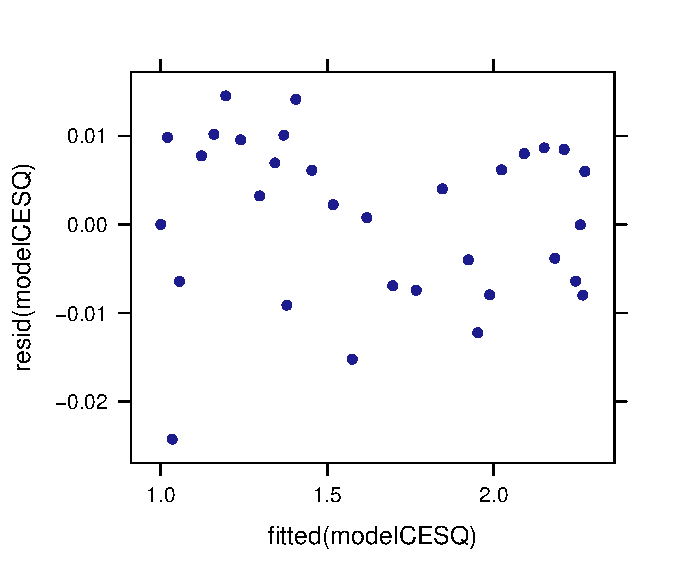
\includegraphics[width=.45\textwidth,height=.38\textwidth]{figure/unnamed-chunk-61} 
\begin{kframe}\begin{alltt}
\hlfunctioncall{histogram}( ~\hlfunctioncall{resid}(modelCESQ) )
\end{alltt}
\end{kframe}
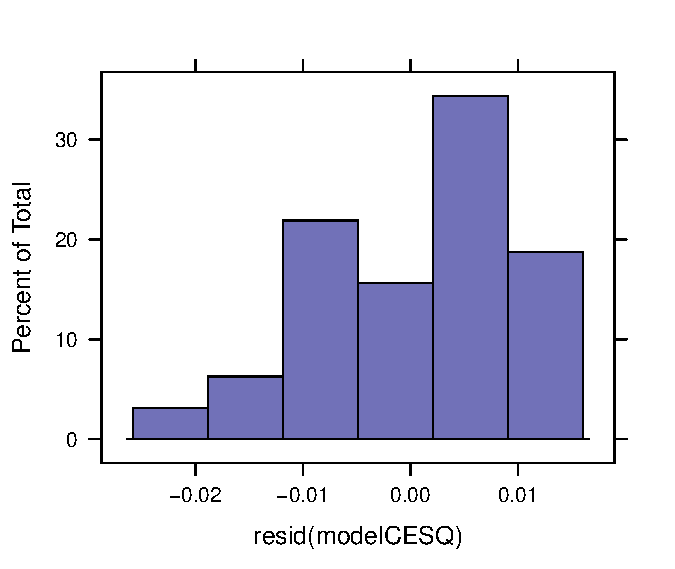
\includegraphics[width=.45\textwidth,height=.38\textwidth]{figure/unnamed-chunk-62} 
\begin{kframe}\begin{alltt}
\hlfunctioncall{qqmath}( ~\hlfunctioncall{resid}(modelCESQ) )
\end{alltt}
\end{kframe}
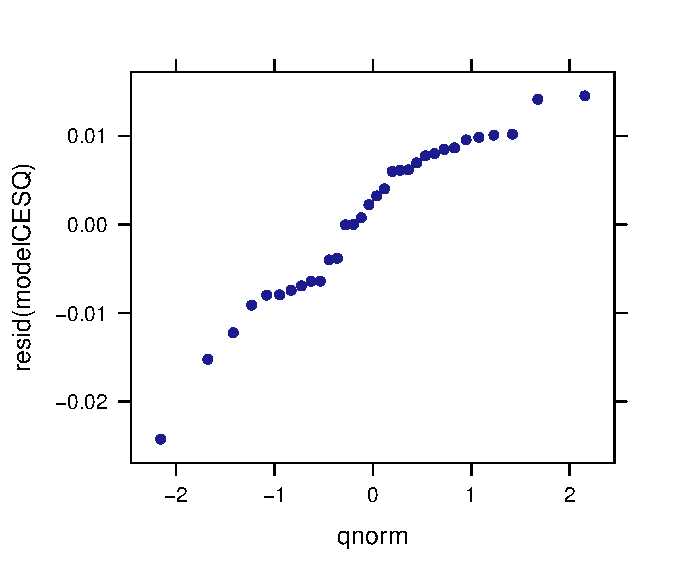
\includegraphics[width=.45\textwidth,height=.38\textwidth]{figure/unnamed-chunk-63} 

\end{knitrout}


%% The Appendices part is started with the command \appendix;
%% appendix sections are then done as normal sections
%% \appendix

%% \section{}
%% \label{}

%% References
%%
%% Following citation commands can be used in the body text:
%%
%%  \citet{key}  ==>>  Jones et al. (1990)
%%  \citep{key}  ==>>  (Jones et al., 1990)
%%
%% Multiple citations as normal:
%% \citep{key1,key2}         ==>> (Jones et al., 1990; Smith, 1989)
%%                            or  (Jones et al., 1990, 1991)
%%                            or  (Jones et al., 1990a,b)
%% \cite{key} is the equivalent of \citet{key} in author-year mode
%%
%% Full author lists may be forced with \citet* or \citep*, e.g.
%%   \citep*{key}            ==>> (Jones, Baker, and Williams, 1990)
%%
%% Optional notes as:
%%   \citep[chap. 2]{key}    ==>> (Jones et al., 1990, chap. 2)
%%   \citep[e.g.,][]{key}    ==>> (e.g., Jones et al., 1990)
%%   \citep[see][pg. 34]{key}==>> (see Jones et al., 1990, pg. 34)
%%  (Note: in standard LaTeX, only one note is allowed, after the ref.
%%   Here, one note is like the standard, two make pre- and post-notes.)
%%
%%   \citealt{key}          ==>> Jones et al. 1990
%%   \citealt*{key}         ==>> Jones, Baker, and Williams 1990
%%   \citealp{key}          ==>> Jones et al., 1990
%%   \citealp*{key}         ==>> Jones, Baker, and Williams, 1990
%%
%% Additional citation possibilities
%%   \citeauthor{key}       ==>> Jones et al.
%%   \citeauthor*{key}      ==>> Jones, Baker, and Williams
%%   \citeyear{key}         ==>> 1990
%%   \citeyearpar{key}      ==>> (1990)
%%   \citetext{priv. comm.} ==>> (priv. comm.)
%%   \citenum{key}          ==>> 11 [non-superscripted]
%% Note: full author lists depends on whether the bib style supports them;
%%       if not, the abbreviated list is printed even when full requested.
%%
%% For names like della Robbia at the start of a sentence, use
%%   \Citet{dRob98}         ==>> Della Robbia (1998)
%%   \Citep{dRob98}         ==>> (Della Robbia, 1998)
%%   \Citeauthor{dRob98}    ==>> Della Robbia


%% References with bibTeX database:

\bibliographystyle{model2-names}
\bibliography{<your-bib-database>}

%% Authors are advised to submit their bibtex database files. They are
%% requested to list a bibtex style file in the manuscript if they do
%% not want to use model2-names.bst.

%% References without bibTeX database:

% \begin{thebibliography}{00}

%% \bibitem must have one of the following forms:
%%   \bibitem[Jones et al.(1990)]{key}...
%%   \bibitem[Jones et al.(1990)Jones, Baker, and Williams]{key}...
%%   \bibitem[Jones et al., 1990]{key}...
%%   \bibitem[\protect\citeauthoryear{Jones, Baker, and Williams}{Jones
%%       et al.}{1990}]{key}...
%%   \bibitem[\protect\citeauthoryear{Jones et al.}{1990}]{key}...
%%   \bibitem[\protect\astroncite{Jones et al.}{1990}]{key}...
%%   \bibitem[\protect\citename{Jones et al., }1990]{key}...
%%   \harvarditem[Jones et al.]{Jones, Baker, and Williams}{1990}{key}...
%%

% \bibitem[ ()]{}

% \end{thebibliography}

\end{document}

%%
%% End of file `elsarticle-template-2-harv.tex'.
